\documentclass[a4paper,12pt]{ctexart}

\usepackage{amsmath}
\usepackage{graphicx}
\usepackage{float}
\usepackage{hyperref}
\usepackage{cite}
\usepackage{algorithm}
\usepackage{algorithmic}
\usepackage{amsmath}
\usepackage{booktabs}
\usepackage{subcaption}
\usepackage{longtable}
\usepackage{amsmath}
\usepackage{array}
\begin{document}


\section{引言}

伪装目标分析(camouflaged object detection)是对一张图片中的伪装目标进行检测或者分割
,而伪装目标则是指所要分析的目标与背景之间存在颜色、纹理、形状等方面的高度相似性,
这种相似性常见于被捕食者改变它们自身的某些特征,使这些特征与周围环境的特征高度相似,从而躲避捕食者的追击。

而与伪装目标分析相对则是显著目标分析(salient object detection),
显著目标分析所要分析的目标与周围环境在颜色、纹理等特征上存在较大的差异,能够被视觉系统快速、精准的捕捉。
一个典型的例子如图\ref{fig:camouflagedVSSalient}所示。

\begin{figure}[htbp]
    \centering
    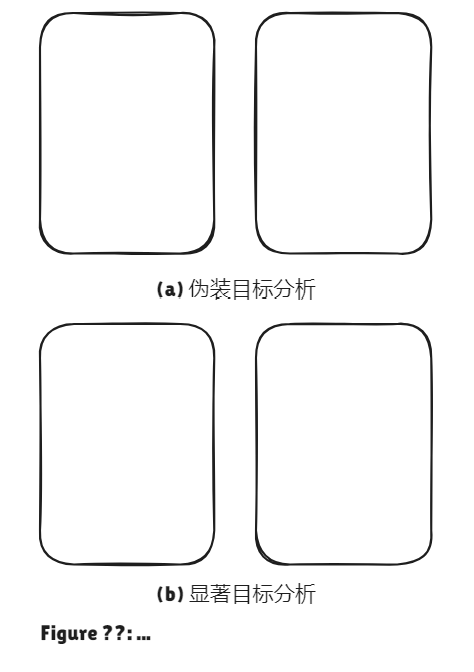
\includegraphics[height=0.5\textheight]{figures/camouflagedVSSalient.png}
    \caption{伪装目标分析与显著目标分析}
    \label{fig:camouflagedVSSalient}
\end{figure}

本报告将围绕伪装目标分割与检测展开,主要使用如下三种方法:
\begin{itemize}
    \item 基于条件随机场(CRF)的伪装目标分割。
    \item 
    \item 
\end{itemize}

\section{相关工作}

\subsection{语义分割}
\textbf{语义分割}是许多视觉理解系统中的核心组成部分,其目的是将图像划分为多个区域。一些早期的方法包括阈值分割\cite{Otsu1979ATS}、基于直方图的分组、区域增长\cite{Nock2004StatisticalRM}、k均值聚类\cite{Dhanachandra2015ImageSU}和分水岭算法\cite{Najman1994WatershedOA}等。这些方法为语义分割奠定了基础,但在复杂场景中往往存在性能限制。近年来,随着深度学习技术的快速发展,语义分割领域迎来了新的变革。深度学习模型通过学习高维特征表示和端到端的优化策略,大幅提升了分割模型的性能。在多个基准数据集上的实验表明,基于深度学习的语义分割方法通常能够取得最高的精度。

\textbf{基于区域分类的语义分割方法} 这一类方法采用自下而上的图像分割方法,生成候选区域后,结合DCNN对分割区域进行分类。例如,在方法\cite{Arbelez2014MultiscaleCG}和\cite{Uijlings2013SelectiveSF}中利用候选边界框和分割区域,将其作为输入提供给DCNN,通过引入形状信息优化分类过程。类似地,\cite{Mostajabi2014FeedforwardSS}采用超像素表示进行区域分割。这些方法能够从高质量的初始分割中受益,但其性能容易受到初始分割的影响,难以实现后续的纠正。

\subsection{伪装目标分割}
\section{方法}

\subsection{基于条件随机场(CRF)的伪装目标分割}

对于任务一,我将采用如下的流程来完成伪装目标分割任务,简要介绍如下:

\begin{enumerate}
    \item \textbf{深度全卷积网络来获取每个像素的初始一元势能(Unary Potential):} 受到DeepLab\cite{Chen2016DeepLabSI}等相关工作的启发,可以利用深度全卷积网络(DCNN)本身对于视觉信息的强大处理能力,直接使用经过预处理的原始图像作为模型输入,来进行一元势能的提取,为后续条件随机场提供一个较好的迭代初始点,详细模型请见\ref{sec:unary}。
    \item \textbf{基于条件随机场(CRF)的后处理逻辑:} 直接使用DCNN的输出作为最终分割掩码可能会导致分割边界粗糙、过多的错误分割区域,分割区域不连续等问题,这些问题出现的根本原因是全卷积网络对于输出像素间的结构关系预测能力较差,而这正是条件随机场模型(CRF)所擅长建模的。条件随机场模型可以基于一些衡量图像像素特征间特定关系的核函数,来对像素类别的可能取值进行更新与约束,从而使预测分割掩码具有一定的结构性,关于条件随机场模型的更多细节请见\ref{sec:crf}。
\end{enumerate}

为了方便起见,我将称该模型为\textbf{DLabCRF}。接下来,我将首先介绍一些观察数据集所得到的发现,随后引出基于这些发现所使用的模型,最后介绍条件随机场模型的后处理逻辑

\subsubsection{基于数据集的发现}
从图\ref{fig:small_dist}可以看出,小伪装目标图片占数据集的绝大部分,这种数据的分布会导致以下问题:
\begin{enumerate}
    \item \textbf{难以分割出较小伪装目标:} 由于伪装目标占整张图片较小的一部分区域,如图\ref{fig:small},且其与周围环境存在颜色与纹理上的高度相似性,所以模型会非常容易将伪装目标误分类成背景。所以对于小尺度上的特征提取就非常重要。DLabCRF利用DeepLab模型所提出的多尺度图像处理以及空洞金字塔池化(ASPP)技巧来缓解该问题所带来的影响。
	\item \textbf{背景部分的预测会主导模型的训练过程:} 对于在包含较小伪装目标的图片上的训练来说,由于伪装类别占整张图片的较小部分,所以用于指导模型参数梯度下降的损失值在平均意义上更偏向于使背景图片分类正确,这样在训练损失值上的体现就是在初期会有一个较大的下降,而在后期保持几乎不变。模型的输出也仅有很小一部分像素,或者没有任何像素,预测为伪装目标。对于该问题的处理,我采用的是基于类别的加权损失计算,即针对伪装目标类别给予较高的权重(0.9),而对于背景类别则是较低的权重(0.1)。
\end{enumerate}

\begin{figure}
    
    \centering
    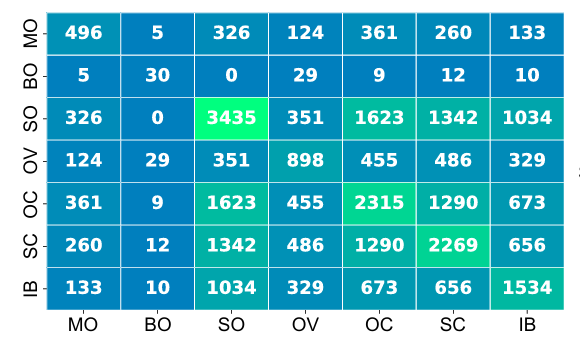
\includegraphics[width=0.5\textwidth]{figures/small_dist.png}
    \caption{\textbf{样本属性分布图} 其中每个单元格表示同时拥有X和Y属性的样本数量,SO表示小伪装目标样本\label{fig:small_dist}}
\end{figure}


\begin{figure}
    \centering
    \begin{subfigure}{0.32\textwidth}
        \centering
        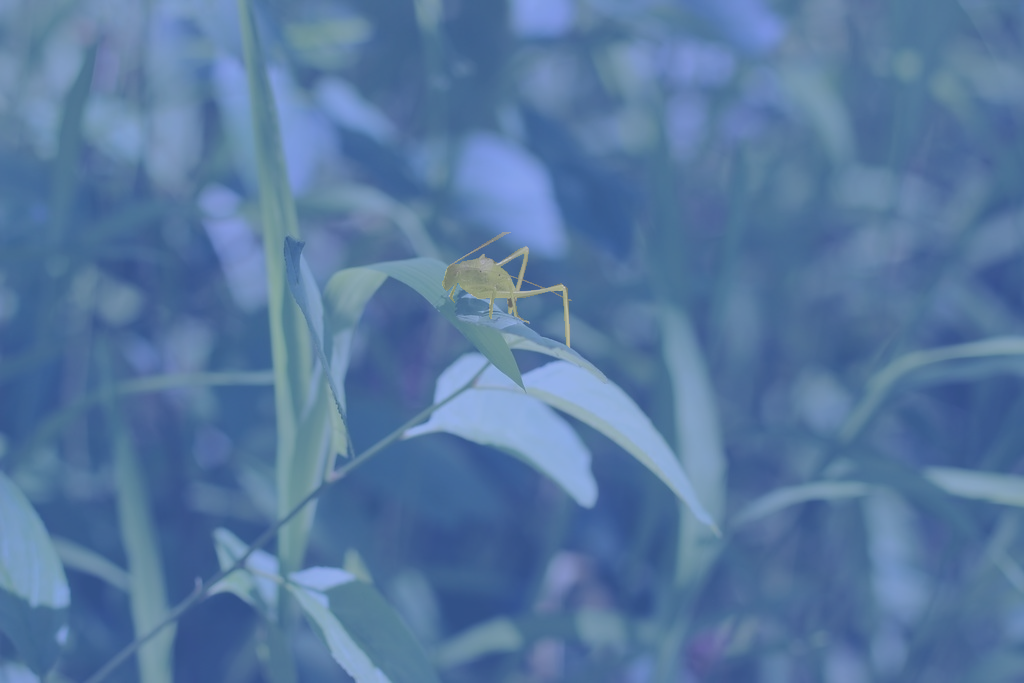
\includegraphics[width=\linewidth]{figures/small_1_resized.png}
    \end{subfigure}%
    \hfill
    \begin{subfigure}{0.32\textwidth}
        \centering
        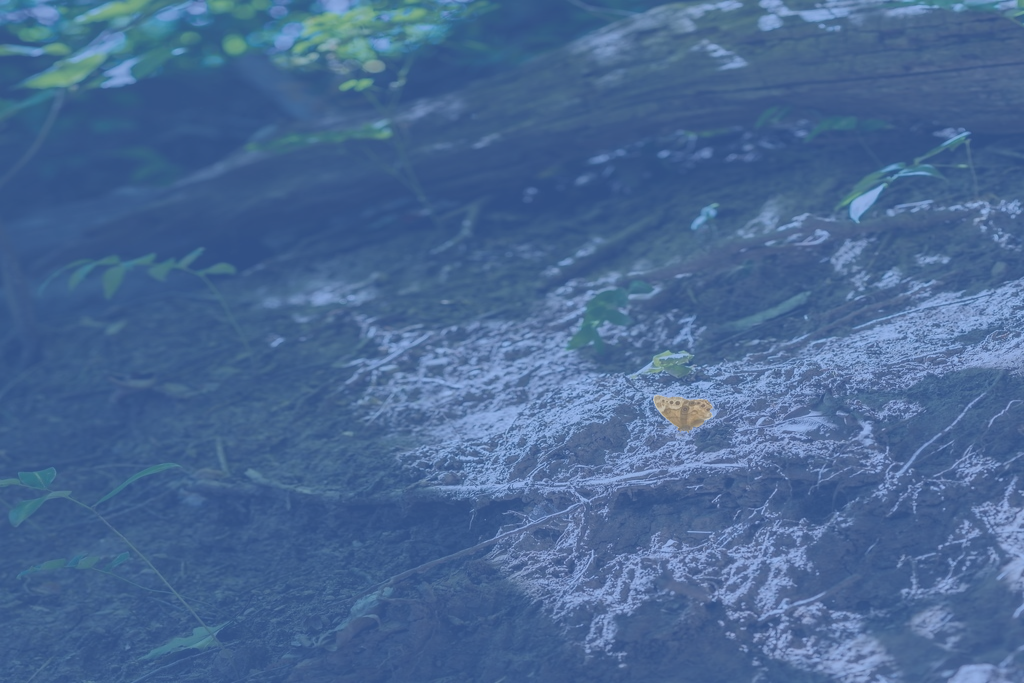
\includegraphics[width=\linewidth]{figures/small_2_resized.png}
    \end{subfigure}
    \hfill
    \begin{subfigure}{0.32\textwidth}
        \centering
        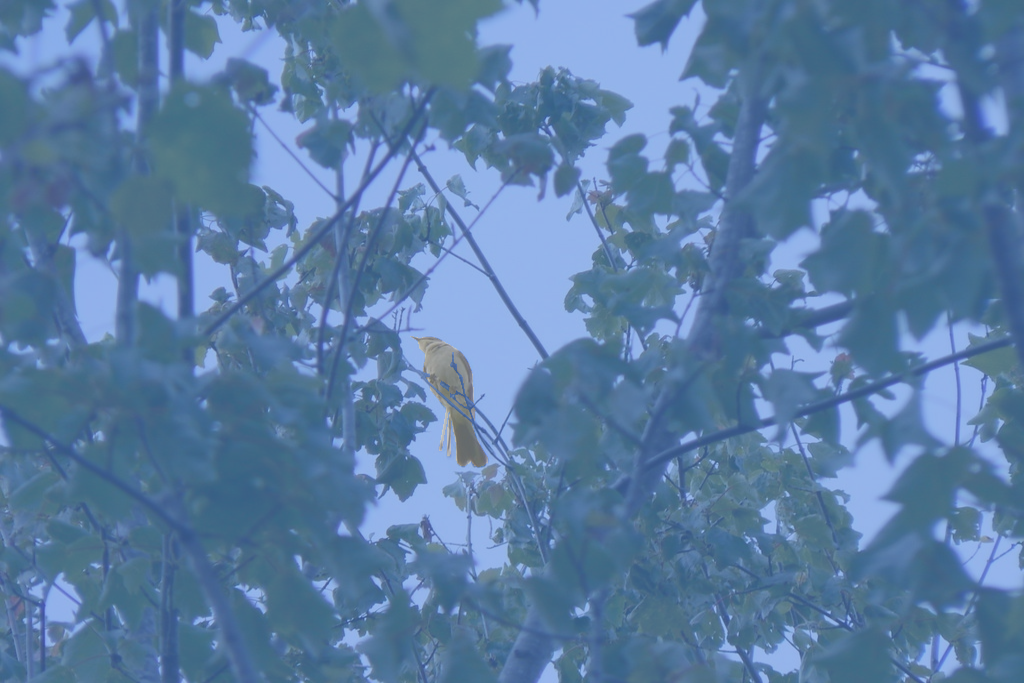
\includegraphics[width=\linewidth]{figures/small_3_resized.png}
    \end{subfigure}%

    \caption{\textbf{小伪装目标图片示例}\label{fig:small}}
\end{figure}

\subsubsection{一元势能提取}
\label{sec:unary}
在本任务中,使用基于Resnet-101的全卷积神经网络\cite{Chen2016DeepLabSI}作为提取一元势能的模块,具体设计细节如下:

\paragraph{空洞卷积的使用:}在深度卷积神经网络(DCNN)中,标准的下采样操作\cite{Shelhamer2014FullyCN}(例如最大池化或步幅卷积)会导致特征图的空间分辨率显著下降。这种降维虽然增强了不变性,但同时降低了空间定位精度,尤其在语义分割任务中会影响对边界和小目标的捕获。为了解决这一问题,DeepLab模型通过在卷积核之间插入“空洞”(即零值)形成空洞卷积来扩大感受野,同时保持特征图的空间分辨率。这种方法无需增加参数量或计算开销,即可在网络中保留更高的分辨率特征。具体实现中,DeepLab 将 ResNet-101 的最后几层池化操作的步幅设为 1,并使用空洞卷积以确保特征响应的密集性,最后使用双边插值将特征图恢复到原始图像分辨率

\paragraph{多尺度分割的处理:}DeepLab模型通过两种方式来处理多尺度分割:
\begin{enumerate}
    \item \textbf{多尺度输入:} 首先通过将输入图像调整为不同的尺寸(如 0.5x、0.75x、1x),然后分别输入到共享参数的 DCNN 中进行特征提取。最后,通过插值将特征图恢复到原始尺寸并采用最大值融合的方式进行多尺度融合。
    \item \textbf{空洞空间金字塔池化(ASPP):} 该模块包含多个并行的分支,每个分支使用不同的空洞率 $r$ 和固定的卷积核(如 $3 \times 3$)。具体设置包括:总共有四个不同的空洞率,分别是6,12,18,24,小空洞率用于捕获细粒度的特征,大空洞率用于捕获全局上下文信息。
\end{enumerate}

在训练阶段,模型分别输出图像在三个尺度下的响应,以及最大值融合响应用于指导训练过程。在推理阶段,模型只输出最大值融合响应作为预测结果,该响应即为条件随机场的一元势能

\subsubsection{基于全连接条件随机场的后处理逻辑}
\label{sec:crf}

在语义分割中,DCNN生成的像素级分类得分图通常是平滑的,但在物体边界处可能会失去细节或出现模糊。为了解决这一问题,可以使用全连接 CRF 模型建模像素间的二元结构关系,增强边界定位并消除伪预测。

\paragraph{能量函数定义}
    全连接 CRF 使用以下能量函数 $E(x)$ 对像素标签分配进行建模:
    $$
    E(x) = \sum_{i} \theta_i(x_i) + \sum_{i,j} \theta_{ij}(x_i, x_j)
    $$
    \begin{itemize}
        \item \textbf{一元势能} $\theta_i(x_i)$:由上述DeepLab的最大值融合响应给出
        \item \textbf{二元势能} $\theta_{ij}(x_i, x_j)$:定义像素 $i$ 和 $j$ 之间的相互作用,旨在通过像素的空间和颜色相似性对分类进行约束。     
    \end{itemize}

\paragraph{二元势能的建模}
    二元势能采用了两种高斯核函数建模像素间关系:
    $$
    \theta_{ij}(x_i, x_j) = \mu(x_i, x_j) \left[ w_1 \exp \left( -\frac{\|p_i - p_j\|^2}{2\sigma_\alpha^2} - \frac{\|I_i - I_j\|^2}{2\sigma_\beta^2} \right) + w_2 \exp \left( -\frac{\|p_i - p_j\|^2}{2\sigma_\gamma^2} \right) \right]
    $$
    \begin{itemize}
    \item 第一项是\textbf{双边核(bilateral kernel)},依赖于像素位置 $p$ 和颜色 $I$,强制空间位置相近且颜色相似的像素拥有相同的标签。
    \item 第二项是\textbf{空间核(spatial kernel)},仅基于像素位置,鼓励空间邻近的像素具有相同标签。
    \item $\mu(x_i, x_j)$ 是 \textbf{Potts 模型},只有当像素 $x_i \neq x_j$ 时,$\mu(x_i, x_j) = 1$,以确保标签不一致时施加惩罚。
    \end{itemize}

\paragraph{推理}
推理过程采用均值场近似以实现高效的推理,更新算法见\ref{alg:meanfield},更新函数如下:
$$
Q_i(Y_i = l) = \frac{1}{Z_i} \exp \left( -\phi_{u,i}(Y_i) - \sum_{l' = 1}^{L} \mu(l, l') \sum_{k=1}^{K} w_k \sum_{j \neq i} g_k(f_i, f_j) Q_j(l') \right)
$$
\begin{algorithm}
    \caption{均值场近似}
    \label{alg:meanfield}
    \begin{algorithmic}[1]
    \STATE $Q_i(Y_i) \leftarrow \frac{1}{Z_i} \exp\left(-\phi_{u,i}(Y_i = l)\right)$ \COMMENT{初始化}
    \WHILE{未收敛}
        \STATE $\hat{Q}_i^k(Y_i = l) \leftarrow \sum_{j \neq i} g_k(f_i, f_j) Q_j(Y_j = l)$ \COMMENT{消息传递}
        \STATE $\tilde{Q}_i(Y_i = l) \leftarrow \sum_{l' \in \mathcal{L}(l, l')} \sum_{k=1}^{K} w_k \hat{Q}_i^k(l')$ \COMMENT{兼容性变换}
        \STATE $Q_i(Y_i) \leftarrow \exp\left(-\phi_{u,i} - \hat{Q}_i(Y_i)\right)$ \COMMENT{局部更新}
        \STATE $Q_i(Y_i) \leftarrow \frac{1}{Z_i} Q_i(Y_i)$ \COMMENT{归一化}
    \ENDWHILE
    \end{algorithmic}
\end{algorithm}

\paragraph{基于贝叶斯优化的参数搜索}
由于CRF在推理过程中,使用参数高斯核函数来建模不同像素特征间的结构关系,所以高斯核函数中参数的取值对最终的分割效果有着较大的影响。故在本节中,讨论基于贝叶斯优化算法的参数搜索策略,以期望找到相对较优的参数组合,从而提高模型的分割性能

首先对条件随机场模型的参数进行定义:
\begin{table}[H]
    \centering
    \begin{tabular}{@{}ll@{}}
    \toprule
    \textbf{参数}       & \textbf{定义}            \\ \midrule
    \texttt{ITER}        & 迭代数                  \\
    \texttt{POS\_W}      & 空间核函数权重          \\
HH]标准差        \H
    \texttt{BI\_W}       & 双边核函数权重          \\
    \texttt{BI\_XY\_STD}  & 双边核函数位置标准差    \\
    \texttt{BI\_RGB\_STD} & 双边核函数颜色标准差    \\ \bottomrule
    \end{tabular}
    \caption{条件随机场模型参数定义}
\end{table}

搜索策略叙述如下:
\begin{enumerate}
    \item 使用一组预设的高斯核函数参数作为初始参数,对迭代数进行实验,迭代数的取值范围是从1到10,观察其对分割性能的影响
    \item 选择最优迭代数固定其不变,对高斯核函数参数进行实验,观察其对分割性能的影响。高斯核函数参数的搜索空间定义如下:
    \begin{table}[H]
    \centering
    \begin{tabular}{@{}lcc@{}}
    \toprule
    \textbf{参数} & \textbf{最小值} & \textbf{最大值} \\ \midrule
    POS\_W            & 1                  & 4                 \\
    POS\_XY\_STD       & 1                  & 10                 \\
    BI\_W             & 1                  & 10                 \\
    BI\_XY\_STD        & 40                 & 60                \\
    BI\_RGB\_STD       & 1                  & 5                 \\ \bottomrule
    \end{tabular}
    \caption{高斯核函数参数搜索空间}
    \end{table}

\end{enumerate}

具体实验结果可以见\ref{sec:crfparam}


\subsection{基于结构支持向量机(SSVM)的伪装目标分割}
结构支持向量机在引入了结构化损失函数之后,可以被用于解决结构化预测问题,即其输出具有某种特定的结构。在任务二中,我将使用基于结构支持向量机的模型来进行伪装目标分割

\subsubsection{模型}
从任务一的结果中可以看到,DLabCRF模型的输出在整体上能够很好的捕捉到伪装目标的整体形状,但是存在以下的问题:
\begin{enumerate}
    \item \textbf{错分类区域:} 即不是伪装目标的区域被分类成伪装目标。这种现象出现的原因是伪装目标与周围环境存在颜色纹理上的高度相似性,导致模型的输出呈现出分割区域分散的问题
    \item \textbf{分割边界模糊且不平滑:} 这是因为DLabCRF底层模型DeepLab本身分割能力的限制以及在最后阶段使用双边插值将分割掩码恢复到真值掩码的大小所导致的
\end{enumerate}

\begin{figure}[h!]
    \centering
    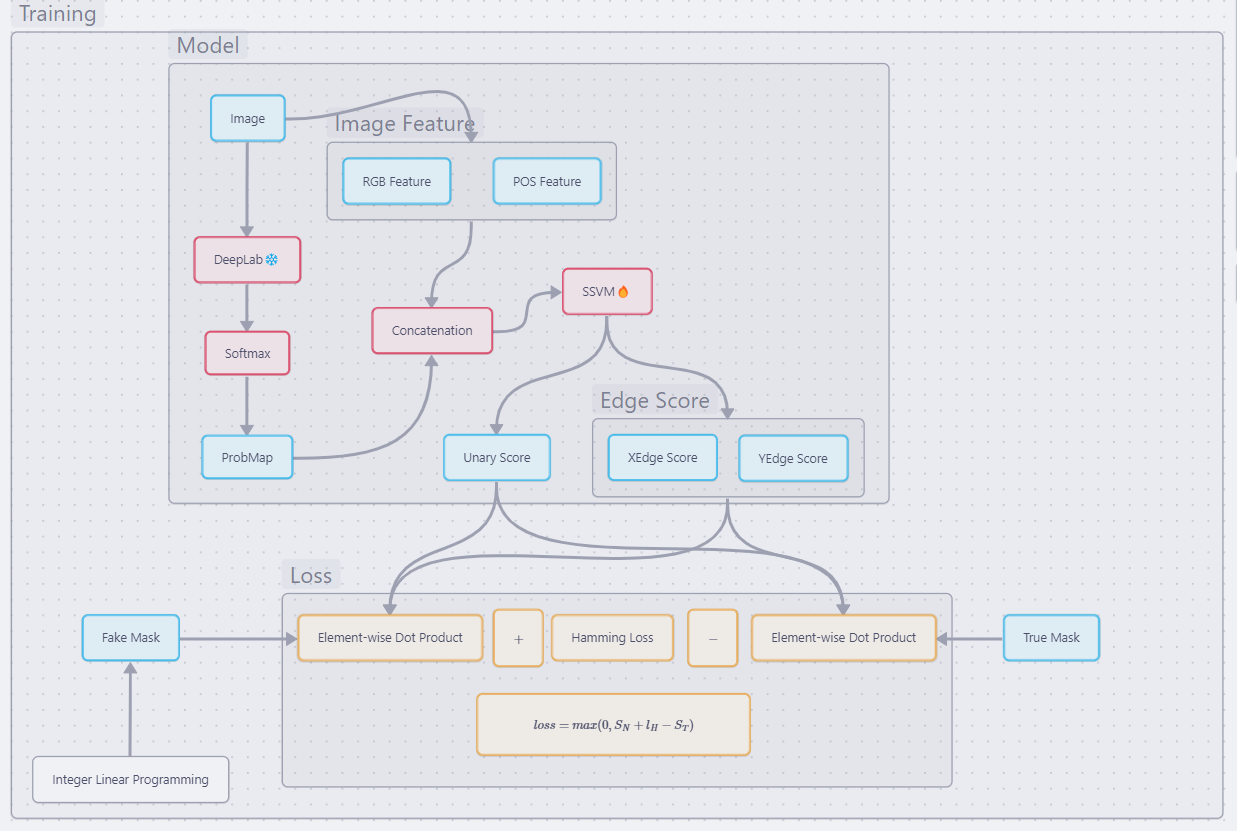
\includegraphics[width=\textwidth]{figures/DLabSSVM/DLabSSVM_training.png}
    \caption{\textbf{DLabSSVM模型结构}\label{fig:DLabSSVM}}
\end{figure}

\begin{figure}[h!]
    \centering
    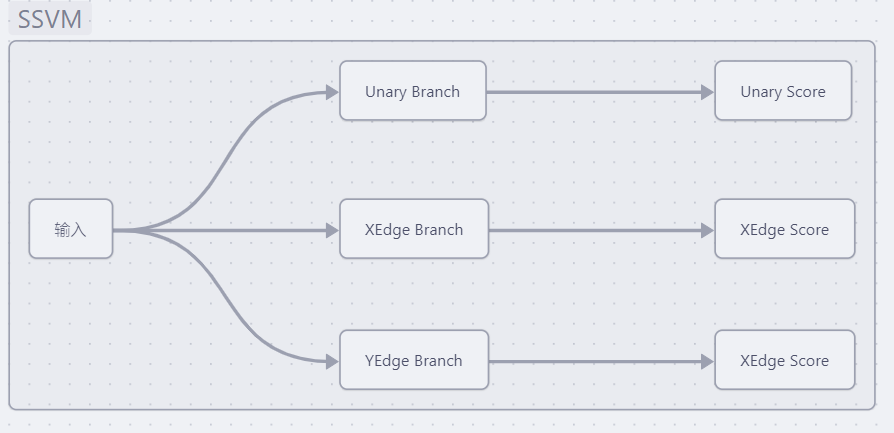
\includegraphics[width=\textwidth]{figures/DLabSSVM/DLabSSVM_ssvm.png}
    \caption{\textbf{SSVM模型结构}\label{fig:SSVM}}
\end{figure}

故在任务二中尝试使用如图\ref{fig:DLabSSVM}的结构,即使用DLabSSVM模型,来尝试解决以上问题,具体细节如下:

\textbf{第一阶段} 该阶段的主要目的是特征提取,使用的仍是DeepLab模型,模型初始化为任务一中预训练的权重,且在之后的训练中不对DeepLab模型的权重进行进一步调整。

DeepLab模型的输出经过softmax函数变为像素点属于某一类别概率的得分图,其通道数为类别数,在伪装类别分析中类别数是2。通过将该得分图与图像的颜色特征以及位置特征进行通道维度上的拼接形成新的特征作为第二阶段结构支持向量机的输入,即每一像素点的特征向量是$(R,G,B,POS\_X,POS\_{Y},S_{1},S_{2})$

\textbf{第二阶段} 该阶段主要目的是使用结构支持向量机对图像像素间的结构关系进行建模。


采用全连接线性层对结构支持向量机进行设计,模型结构可见图\ref{fig:SSVM}。具体来说,结构支持向量机有三个分支,每个分支模型都采用全连接线性层设计:
\begin{enumerate}
    \item \textbf{Unary Branch:} 该分支负责输出像素点一元得分图,即该分支只考虑像素点自身的特征,输出的得分图中每一像素是该像素点属于每一类别的得分。
    \item \textbf{XEdge Branch:} 该分支接受当前像素点与其右侧的第一个像素点拼接形成的向量作为输入,输出是在水平X方向上像素间的二元得分图
    \item \textbf{YEdge Branch:} 该分支接受当前像素点与其下侧的第一个像素点拼接形成的向量作为输入,输出是在垂直Y方向上像素间的二元得分图
\end{enumerate}

\subsubsection{训练}

DLabSSVM模型所要训练的只有结构支持向量机模块。训练流程包括以下两个部分:
\begin{enumerate}
    \item \textbf{伪掩码的产生:} 这里的伪掩码指的是得分高且与真值掩码差异较大的分割掩码,该掩码用整数线性规划求解,具体细节可见\ref{sec:ILP}。
    \item \textbf{结构化铰链损失(Structural Hinge Loss):} 利用如下函数计算伪掩码和真值掩码的得分:
\end{enumerate}
	$$
	Score(Mask,\,SMap) = \sum_{i}^3 Dot(Mask_{i},SMap_{i})
$$
	即计算掩码与三个得分图的点积并相加。分别记伪掩码得分为$S_{N}$,真值掩码得分为$S_{T}$,代入如下的结构化铰链损失函数:
	$$
L_{\text{structural}}(x, \hat{y}, y) = \max \left( 0, l_{h}(y, \hat{y}) - S_{T} + S_{N} \right)
$$
	其中$l_{h}$为汉明损失。
随后可用得到的损失值进行梯度计算,从而实现模型训练

\subsubsection{推理}

\begin{figure}[h!]
    \centering
    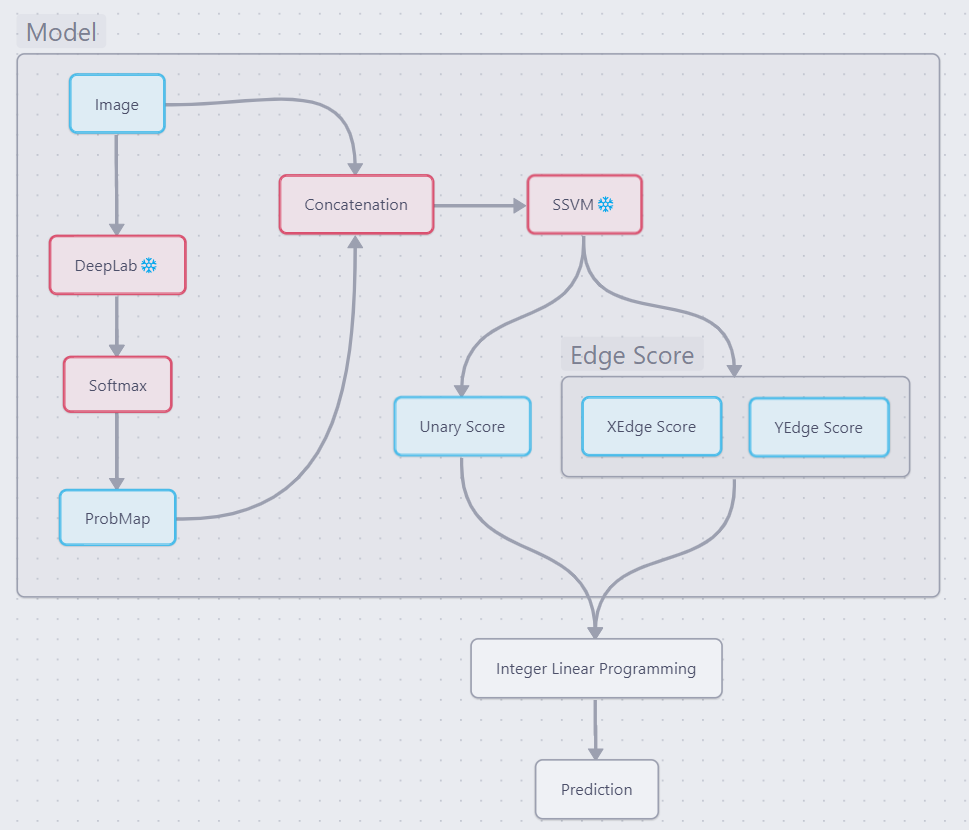
\includegraphics[width=\textwidth]{figures/DLabSSVM/DLabSSVM_inference.png}
    \caption{模型推理结构\label{fig:inference}}
\end{figure}

模型推理流程可见图\ref{fig:inference}。通过在预测的得分图上进行整数线性规划,从而得到约束条件下的最佳分割掩码。

\subsubsection{整数线性规划}
\label{sec:ILP}
在DLabSSVM中,整数线性规划(Integer Linear Programming)被分别用在训练阶段中的伪掩码的产生以及推理阶段预测掩码的产生,两个过程的本质都是求解如下的整数线性规划问题:
$$
\begin{cases}
x_{ijc} = 0 \text{ or } 1, & i \in \{1, \dots, H\}, j \in \{1, \dots, W\}, c = 0 \text{ or } 1 \\
e_{ijc}^1 = 0 \text{ or } 1, & i \in \{1, \dots, H\}, j \in \{1, \dots, W-1\}, c = 0 \text{ or } 1 \\
e_{ijc}^2 = 0 \text{ or } 1, & i \in \{1, \dots, H-1\}, j \in \{1, \dots, W\}, c = 0 \text{ or } 1
\end{cases}
$$
约束条件:
$$
\text{s.t.} \quad 
\begin{cases}
\sum_{k=0}^{c} X_{ijc} = 1 \\
e_{ijc}^1 \leq X_{ijc} \\
e_{ijc}^1 \leq X_{i(j+1)c} \\
e_{ijc}^2 \leq X_{ijc} \\
e_{ijc}^2 \leq X_{(i+1)jc}
\end{cases}
$$
在训练阶段使用损失增强的\textbf{最大后验推理(loss augmentated MAP inference)},即最大化如下目标函数:
$$
\text{obj} = \sum_{i=1}^3 Dot(Mask_{i},SMap_{i}) + \sum l(y, X)
$$
其中$Mask_{1}=x,Mask_{2}=e^1,Mask_{3}=e^2$,$l(\cdot)$为汉明损失,该目标函数保证所选择的是模型最容易混淆的掩码,即与真值掩码差异最大(最大化汉明损失),且得分最高的掩码。

在推理测段只需要保证预测掩码得分最高即可,即最大化如下目标函数:
$$
\text{obj} = \sum_{i=1}^3 Dot(Mask_{i},SMap_{i})
$$

\subsection{基于AdaBoost的伪装目标识别}

\section{实验}

\subsection{数据集}
\paragraph{CAMO\cite{Le2019AnabranchNF}:}该数据集中总共有1250张,取该数据集的前1055个样本作为训练数据CAMO\_Train,之后的195个样本按照1:1的比例分为验证集CAMO\_VAL和测试集CAMO\_TEST

\paragraph{COD10k\cite{Fan2020CamouflagedOD}: }该数据集包含5066张伪装目标图片,3000张背景图片,1934张非伪装目标图片。类别划分为5个超类,78个子类,并且对于每一张伪装目标图片都标注有关键特征(如多目标、小目标、有遮盖,形状复杂等)。对前55个子类样本组成的数据集进行抽样,所形成的新的数据集作为训练数据COD10K\_Train,共2900张图片。对后23个子类进行同样的处理,所形成的数据集有1100图片,按照1:1比例分为验证集COD10K\_VAL和测试集COD10K\_TEST。

数据划分如下:
\begin{table}[ht]
    \centering
    \begin{tabular}{|c|c|}
    \hline
    \textbf{划分} & \textbf{数据集} \\
    \hline
    训练集 & CAMO\_Train + COD10K\_Train \\
    \hline
    验证集 & CAMO\_VAL + COD10K\_VAL \\
    \hline
    测试集 & CAMO\_TEST \\
          & COD10K\_TEST \\
    \hline
    \end{tabular}
    \caption{数据集划分}
\end{table}
\subsection{评价指标}

\subsection{伪装目标分割实验结果分析}
\subsubsection{模型训练分析}

\begin{figure}[h!]
    \centering
    \begin{subfigure}{0.4\textwidth}
        \centering
        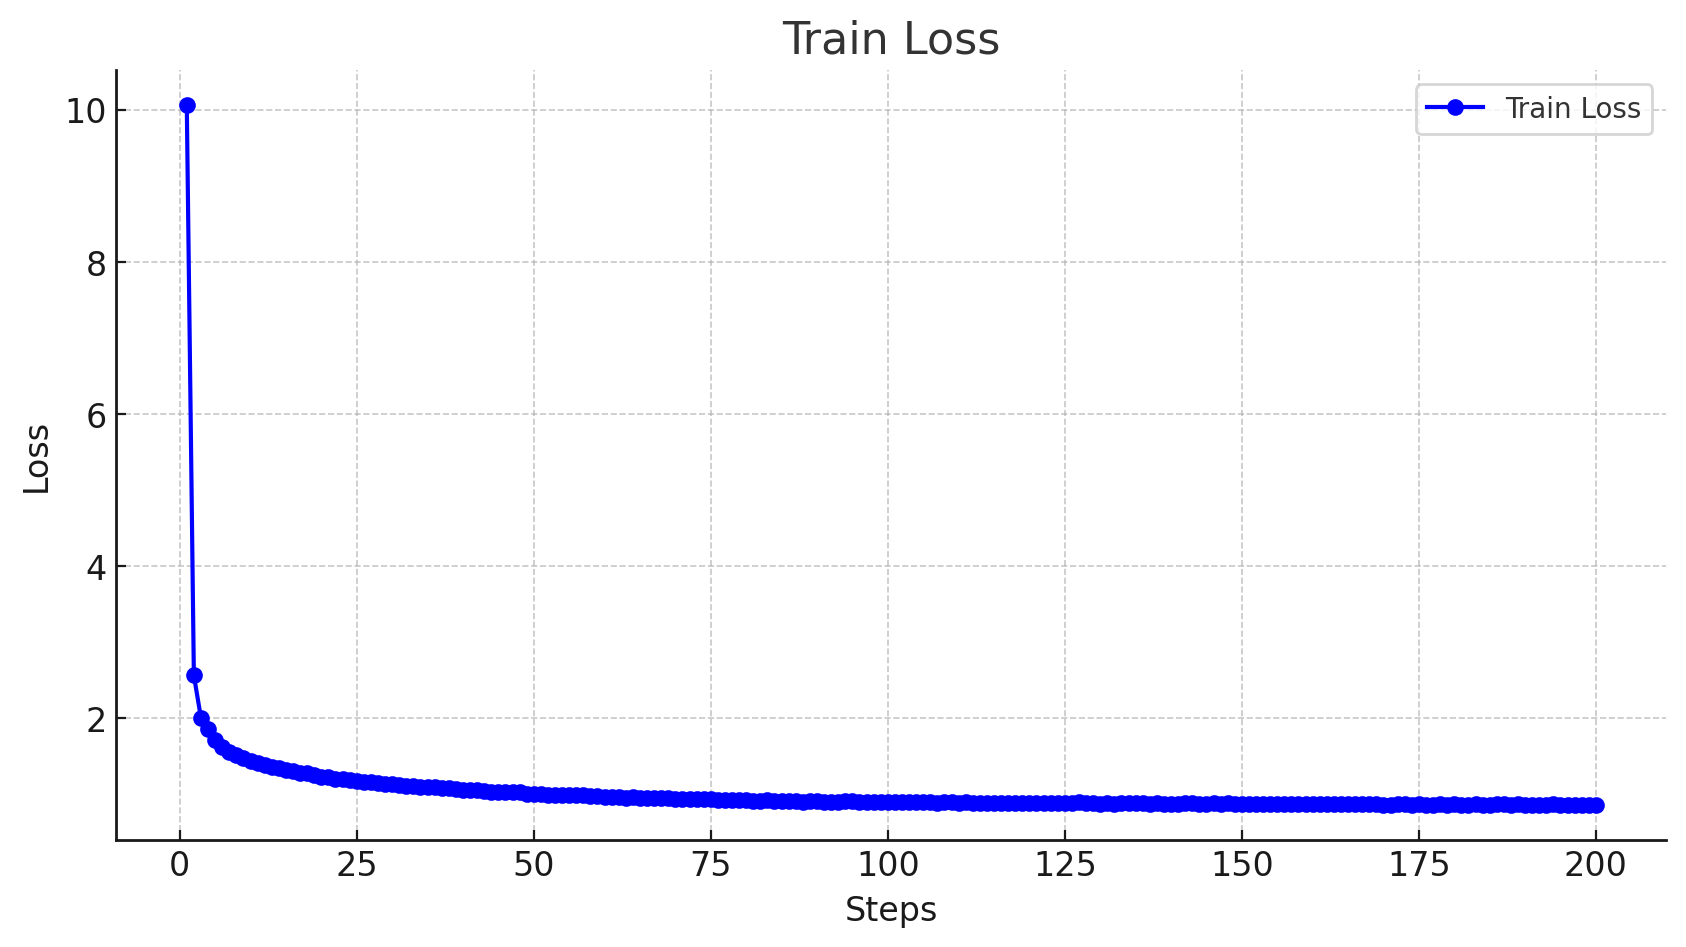
\includegraphics[width=\linewidth]{figures/deeplab_train_loss.png}
        \caption{DeepLab训练损失}
        \label{fig:dlabloss}
    \end{subfigure}%
    \hspace{0.1\textwidth}
    \begin{subfigure}{0.4\textwidth}
        \centering
        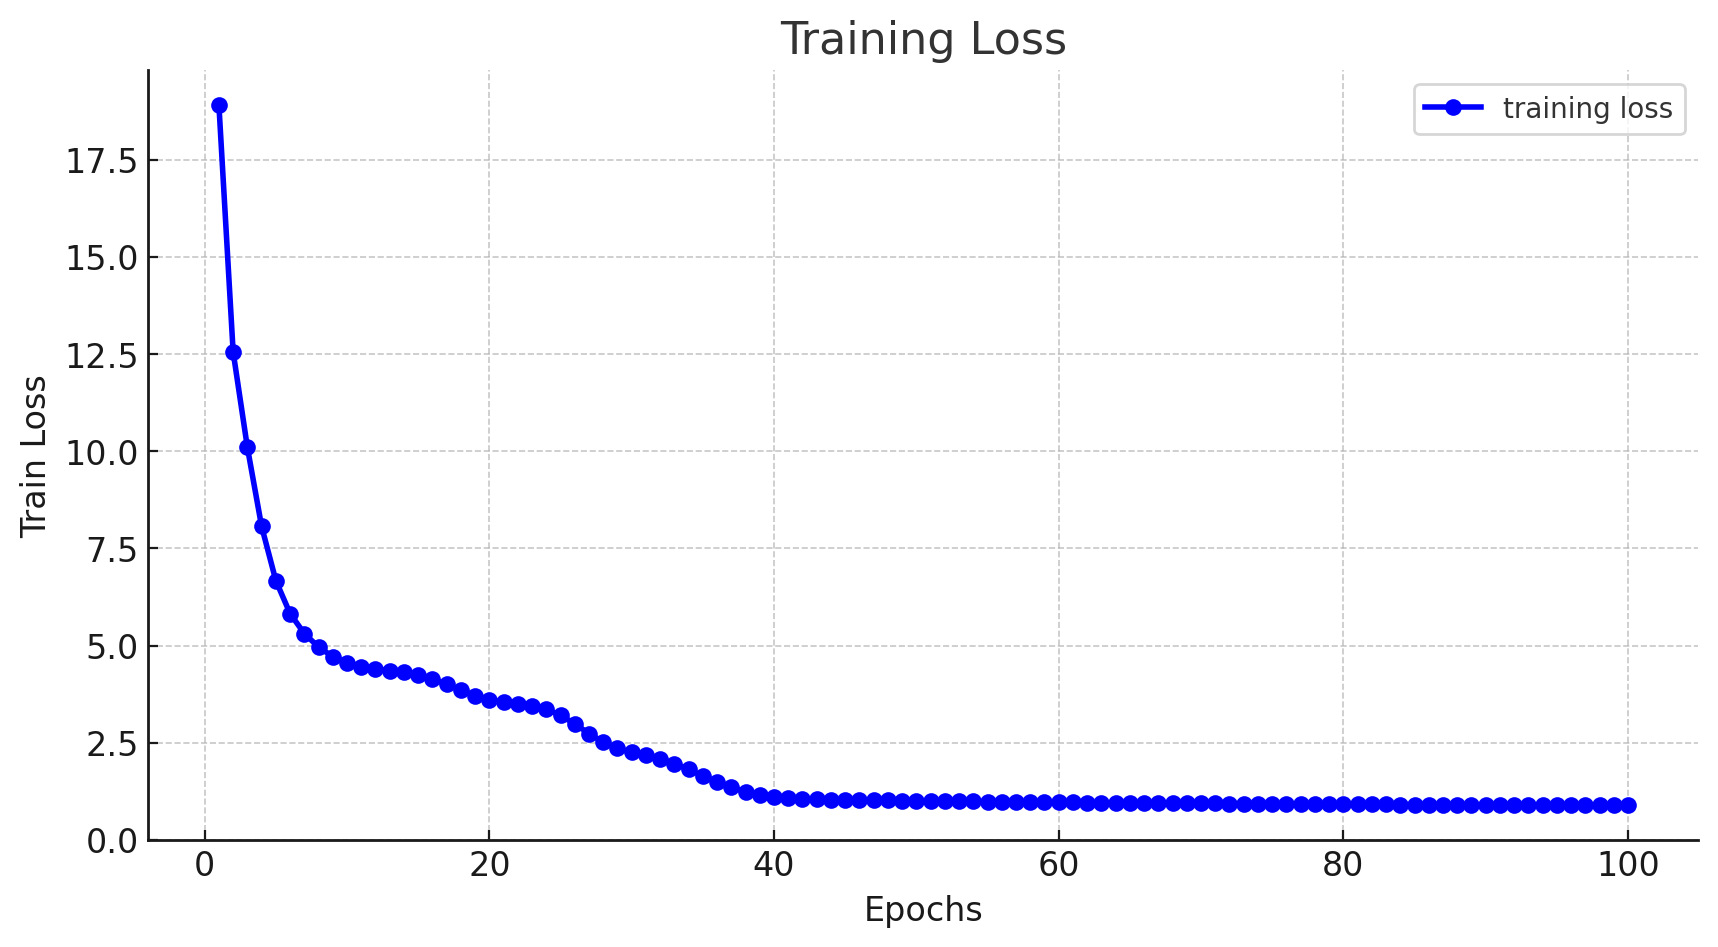
\includegraphics[width=\linewidth]{figures/ssvm_train_loss.png}
        \caption{DLabSSVM训练损失}
        \label{fig:dssvmloss}
    \end{subfigure}%
    \hspace{0.1\textwidth}
    \begin{subfigure}{0.4\textwidth}
        \centering
        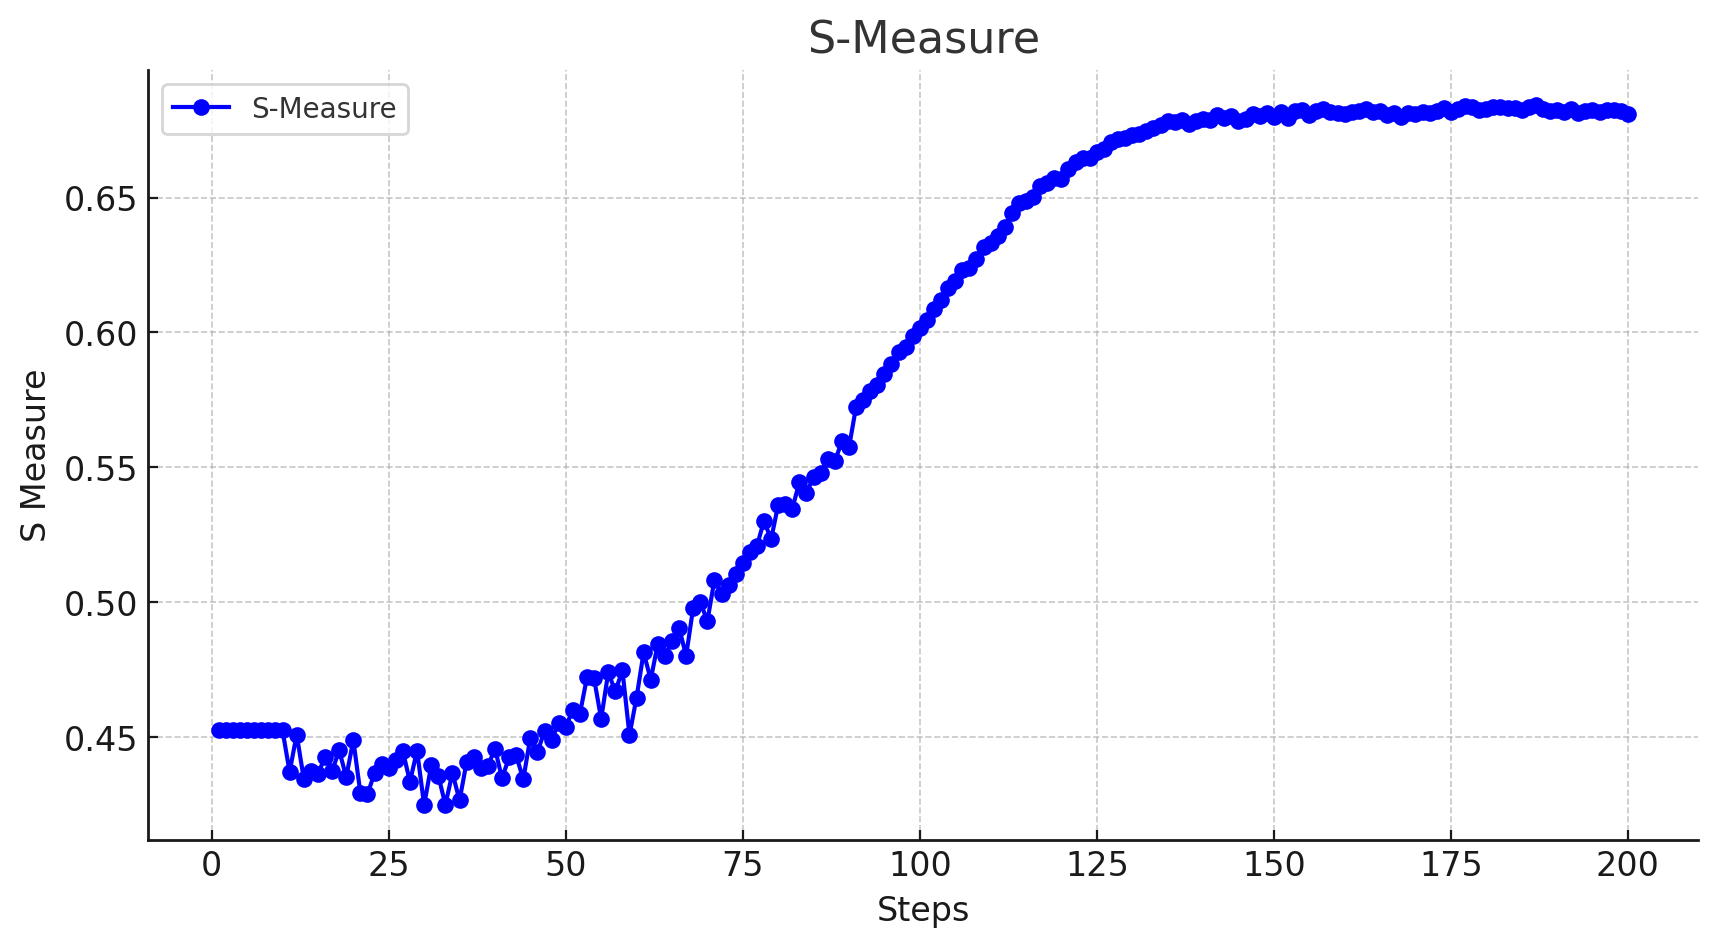
\includegraphics[width=\linewidth]{figures/deeplab_smeasure.png}
        \caption{DeepLab结构度量}
        \label{fig:dlabsm}
    \end{subfigure}%
    \hspace{0.1\textwidth}
    \begin{subfigure}{0.4\textwidth}
        \centering
        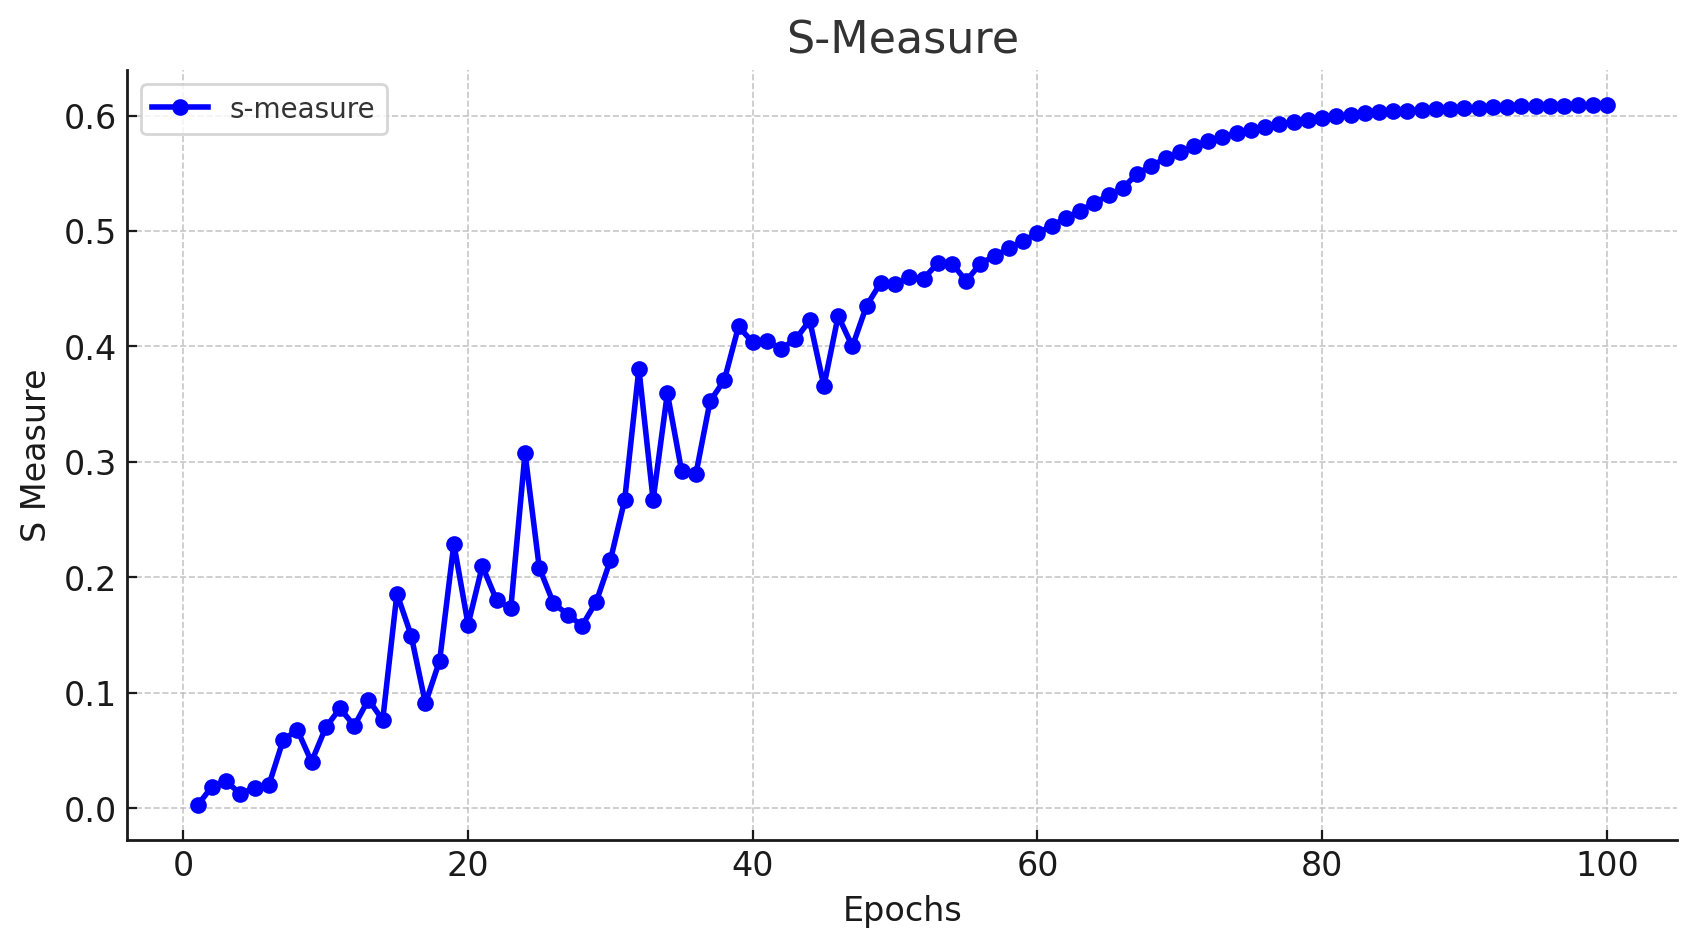
\includegraphics[width=\linewidth]{figures/ssvm_smeasure.png}
        \caption{DLabSSVM结构度量}
        \label{fig:dssvmsm}
    \end{subfigure}%
\end{figure}

在伪装目标切割任务中,需要训练的模块有两个,一个是用于特征提取的DeepLab模型,另一个是DLabSSVM中用于结构化预测的SSVM模型。现在从训练过程中的指标变化来深入分析这两个模型的表现:

\paragraph{训练损失}如\ref{fig:dlabloss}和\ref{fig:dssvmloss}所示,在训练初期,DeeLab模型的损失值呈现出急剧下降的趋势,尤其是在训练的前几步,损失从接近10迅速降到接近2,但DLabSSVM模型相较于DeepLab模型下降较缓,在30个epochs左右降至5,并在后期趋于平稳。

\paragraph{结构度量}从\ref{fig:dlabsm}和\ref{fig:dssvmsm}中可以看出,与DLabSSVM模型的初期结构度量相比,DeepLab模型在前期的结构度量值较高(约为0.45),这是因为DeepLab模型使用了在COCO和PASCAL VOC数据集上预训练的权重,导致其在最开始阶段有一个相当不错的准确率,但DLabSSVM中的SSVM模块是随机初始化权重,所以在刚开始训练阶段的结构度量并没有DLabCRF出色。
随着训练的推进,两者的结构度量值都在稳步上升,最终DeepLab稳定在0.68左右,而DLabSSVM则稳定在0.61左右。





\subsubsection{模型性能对比}

\begin{table}[h!]
    \centering
    \begin{tabular}{|l|c|c|c|c|}
    \hline
    \textbf{Model} & \multicolumn{2}{c|}{\textbf{CAMO Test}} & \multicolumn{2}{c|}{\textbf{COD10K Test}} \\
    \cline{2-5}
     & \textbf{MAE} & \textbf{S-Measure} & \textbf{MAE} & \textbf{S-Measure} \\
    \hline
    Deeplab & 0.134 & \textbf{0.688} & 0.064 & 0.693 \\
    DLabCRF & \textbf{0.133} & 0.685 & \textbf{0.057} & \textbf{0.706} \\
    DLabSSVM & 0.191 & 0.607 & 0.124 & 0.637 \\
    \hline
    \end{tabular}
    \caption{伪装目标分割模型性能对比}
\end{table}

从在两个测试集上的性能来看,DLabCRF模型在整体上优于DeepLab模型,尤其是在COD10K Test数据集上。
这可能是因为CRF通过均值场近似算法将DeepLab模型预测与像素点的颜色和位置信息进行了整合
从而使得原先的离散的分割区域得到了合并,边界变得更加平滑,从而提高了分割的准确性。

而SSVM模型的性能相对较差,可能有以下几个原因:
\begin{enumerate}
    \item \textbf{SSVM结构过于简单:} SSVM结构设计采用深度较浅的全连接线性层,无法有效的捕捉到像素间的结构关系,存在结构信息丢失的问题
    \item \textbf{推理算法的选择:} 因为DLabSSVM使用整数线性规划(ILP)来进行推理,故为了保证训练过程的可行性与高效性,
    即在训练时能够在有限时间内找到约束条件下的最具代表性的伪掩码进行指导训练,我通过将得分图的分辨率进行降低,并在最后使用插值的方式将分割掩码恢复到原始分辨率,
    这样的处理方式可能会导致分割掩码的边界模糊,离散伪分割区域较多等问题,这一点在\ref{sec:visual}中也可以看出来。
    \item \textbf{像素间结构关系的建模过于简单:} 我只考虑了像素与其右侧和下侧的第一个像素间的关系,这种建模方式
    易于实现,但是对于像素间的结构关系捕捉不够充分,导致DLabSSVM模型的性能在DeepLab模型之下。
\end{enumerate}

\subsubsection{不同CRF参数下的性能指标对比}
\label{sec:crfparam}

\[\begin{array}{|c|c|c|c|c|c|c|c|c|c|}
    \hline
    \text{Iteration} & 0 & 1 & 2 & 3 & 4 & 5 & 6 & 7 & 8 \\
    \hline
    \text{S-Measure} & 0.689 & 0.695 & 0.693 & 0.693 & 0.692 & 0.691 & 0.689 & 0.688 & 0.685 \\
    \hline
\end{array}
\]

从上表中可以得到CRF均值随机场迭代次数越少,结构度量值S-Measure越高。但同时从迭代次数为0和非0时的对比中,即有无CRF后处理逻辑,可以证明CRF模块在提升分割精度上的有效性

\begin{figure}[h]
    \centering
    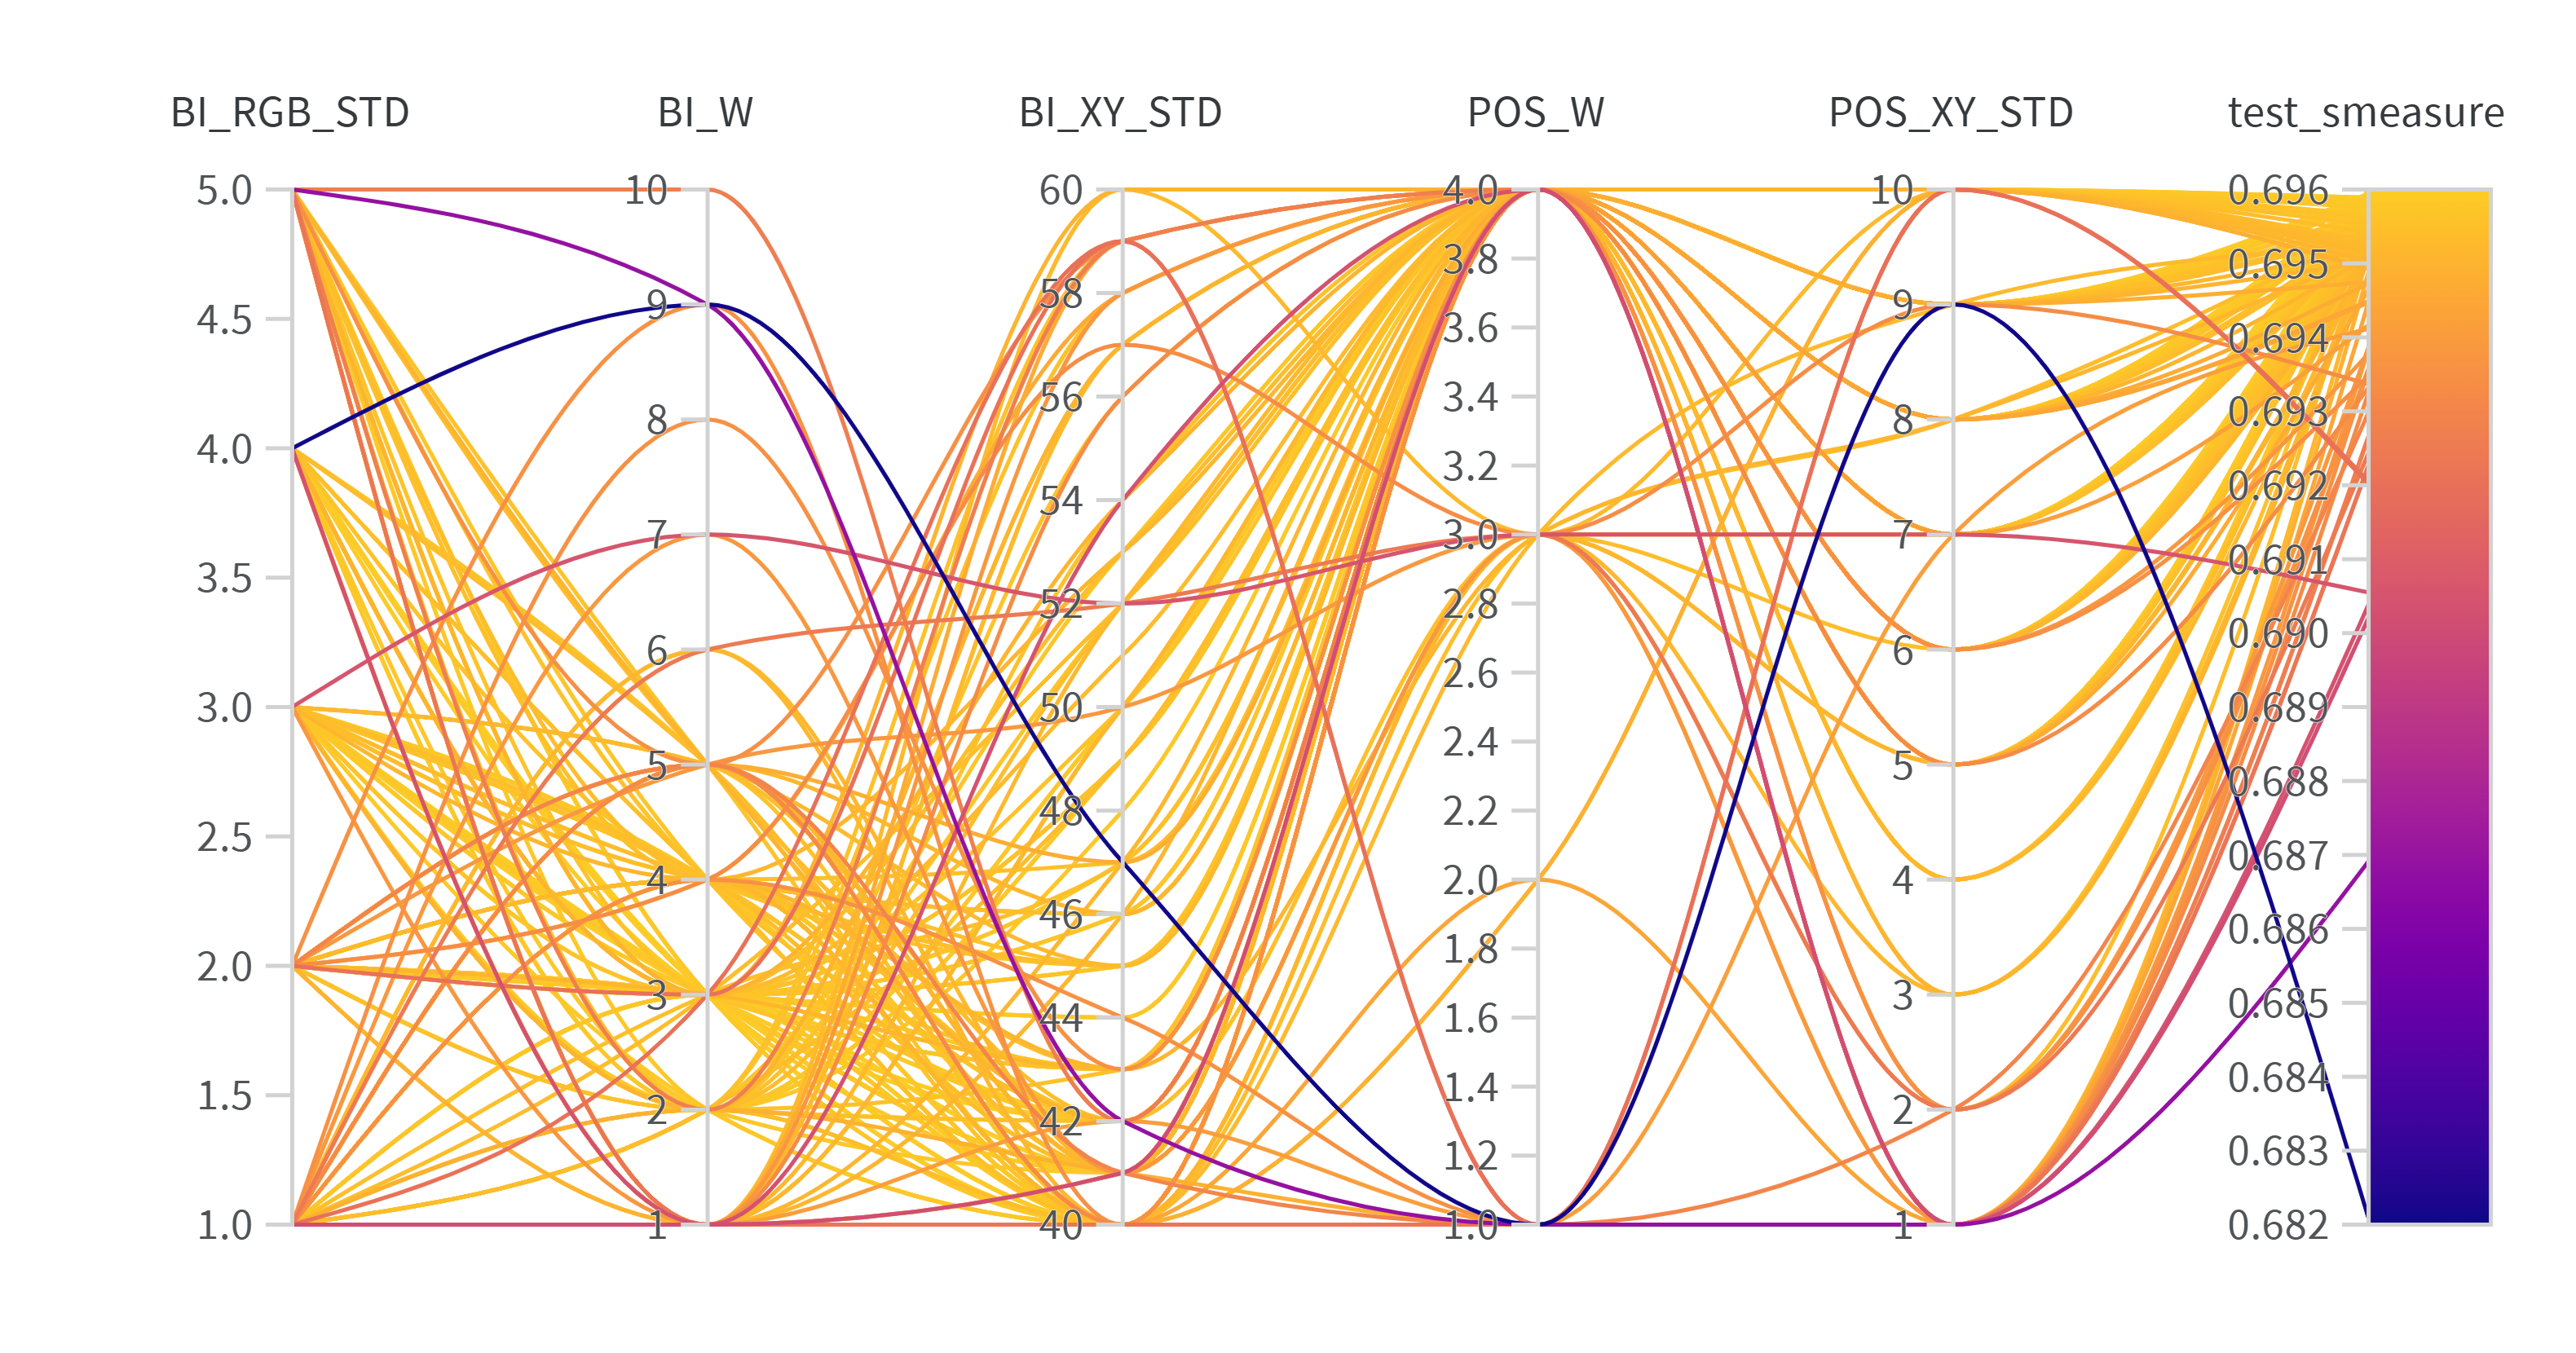
\includegraphics[width=\textwidth]{figures/crfparam_search.png}
    \caption{CRF参数搜索}
    \label{fig:crfps}
\end{figure}

固定CRF迭代次数为1,对高斯核函数的参数进行搜索,得到如图\ref{fig:crfps}所示的平行坐标图。其中当参数取以下值时,结构度量值得到最大0.696,故选取该组参数作为后续实验的CRF参数。

\[\begin{array}{|c|c|c|c|c|c|c|c|c|c|}
    \hline
    \text{Iter} & $POS\_W$ & $POS\_XY\_STD$ & $BI\_W$ & $BI\_XY\_STD$ & $BI\_RGB\_STD$ \\
    \hline
    1 & 4 & 7 & 3 & 40 & 4 \\
    \hline
\end{array}
\]

\subsubsection{可视化分析}
\label{sec:visual}


\begin{figure}[h]
    \centering
    \begin{subfigure}{0.5\textwidth}
        \centering
        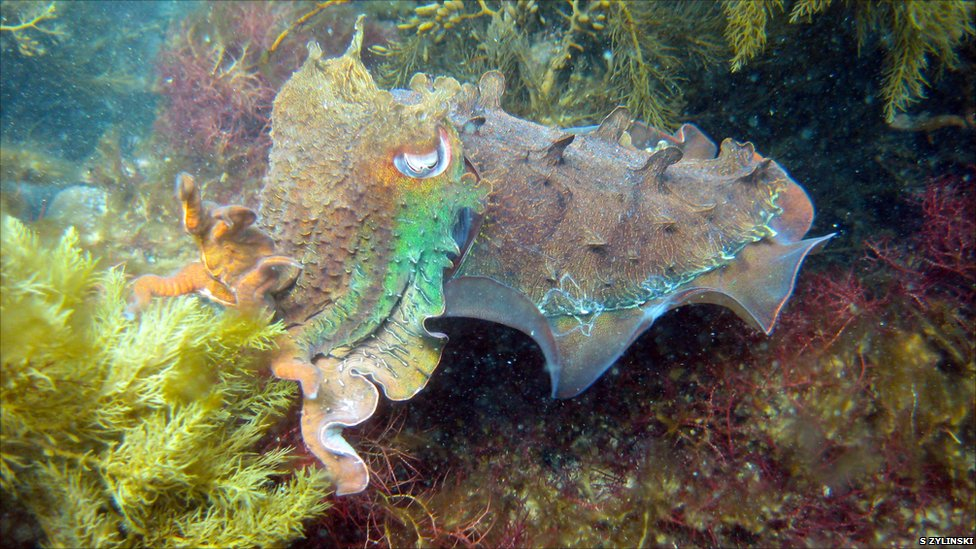
\includegraphics[width=\linewidth]{figures/CAMO_demo1/CAMO_demo1_ori.png}
        \label{fig:demo1_ori}
    \end{subfigure} \\

    \begin{subfigure}{0.25\textwidth}
        \centering
        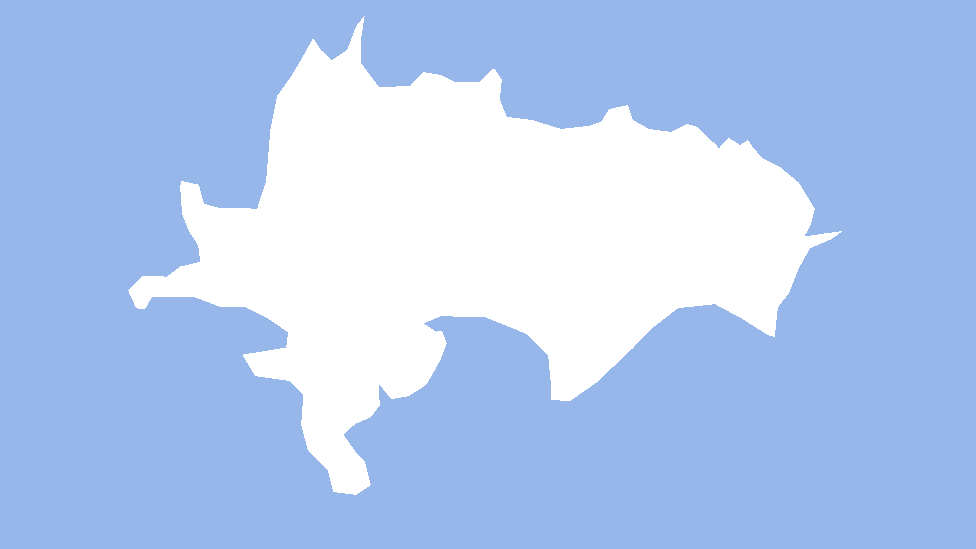
\includegraphics[width=\linewidth]{figures/CAMO_demo1/CAMO_demo1_gt.png}
        \label{fig:demo1_gt}
        \caption{Ground Truth}
    \end{subfigure}%
    \hfill
    \begin{subfigure}{0.25\textwidth}
        \centering
        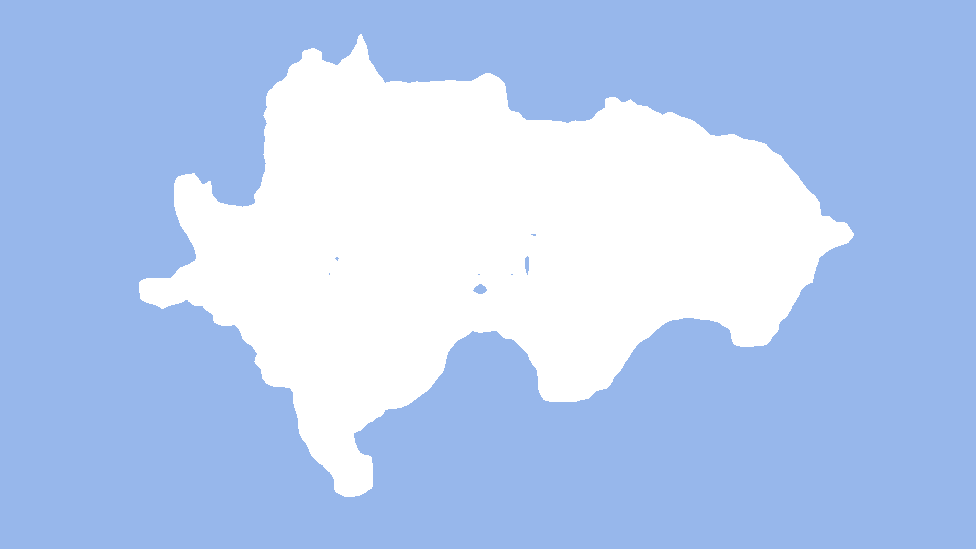
\includegraphics[width=\linewidth]{figures/CAMO_demo1/CAMO_demo1_pred_ssvm.png}
        \label{fig:demo1_dlap}
        \caption{DeepLab}
    \end{subfigure}%
    \hfill
    \begin{subfigure}{0.25\textwidth}
        \centering
        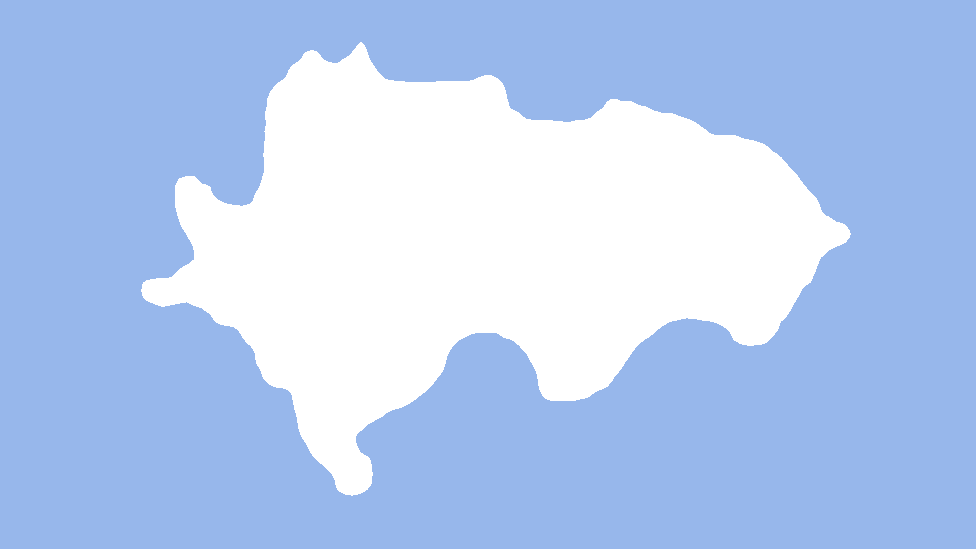
\includegraphics[width=\linewidth]{figures/CAMO_demo1/CAMO_demo1_pred_crf.png}
        \label{fig:demo1_crf}
        \caption{DLabCRF}
    \end{subfigure}%
    \hfill
    \begin{subfigure}{0.25\textwidth}
        \centering
        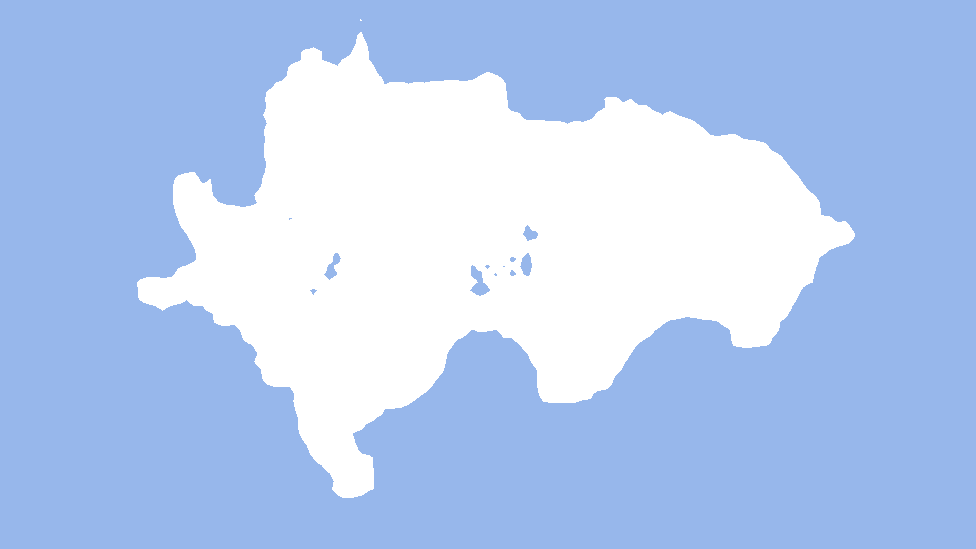
\includegraphics[width=\linewidth]{figures/CAMO_demo1/CAMO_demo1_pred_dlap.png}
        \label{fig:demo1_ssvm}
        \caption{DLabSSVM}
    \end{subfigure}

    \caption{CAMO 可视化 \label{fig:CAMO_demo1}}
\end{figure}

\begin{figure}[h]
    \centering
    \begin{subfigure}{0.4\textwidth}
        \centering
        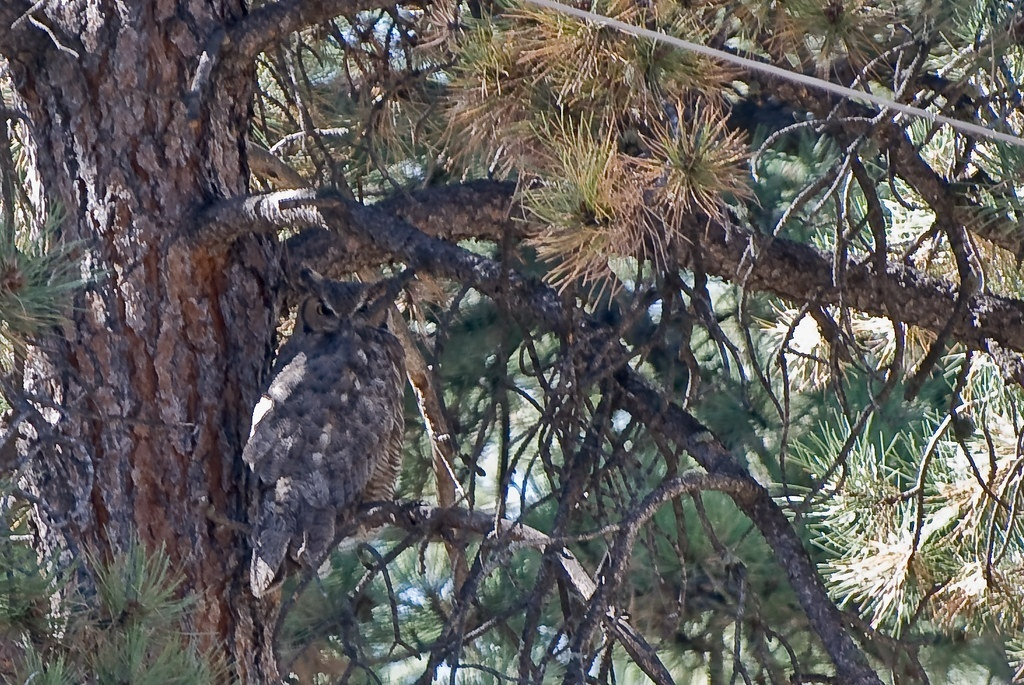
\includegraphics[width=\linewidth]{figures/COD10K_demo1/COD10K_demo1_ori.png}
    \end{subfigure} \\

    \begin{subfigure}{0.25\textwidth}
        \centering
        
\includegraphics[width=\linewidth]{figures/COD10K_demo1/COD10K_demo1_gt.png}
        \caption{Ground Truth}
    \end{subfigure}%
    \hfill
    \begin{subfigure}{0.25\textwidth}
        \centering
        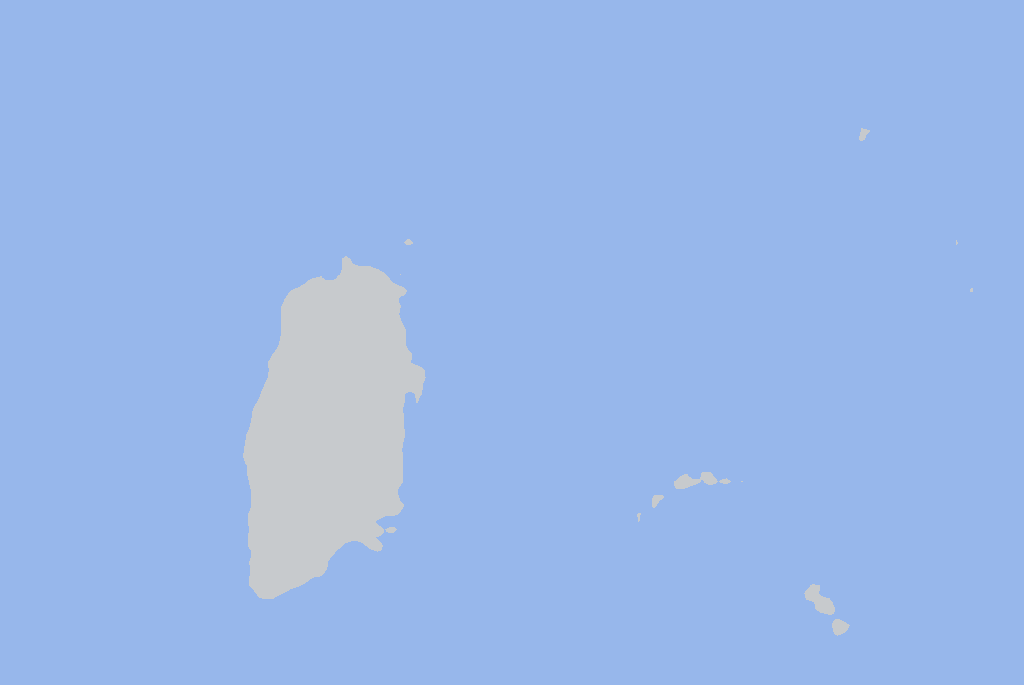
\includegraphics[width=\linewidth]{figures/COD10K_demo1/COD10K_demo1_pred_ssvm.png}
        \caption{DeepLab}
    \end{subfigure}%
    \hfill
    \begin{subfigure}{0.25\textwidth}
        \centering
        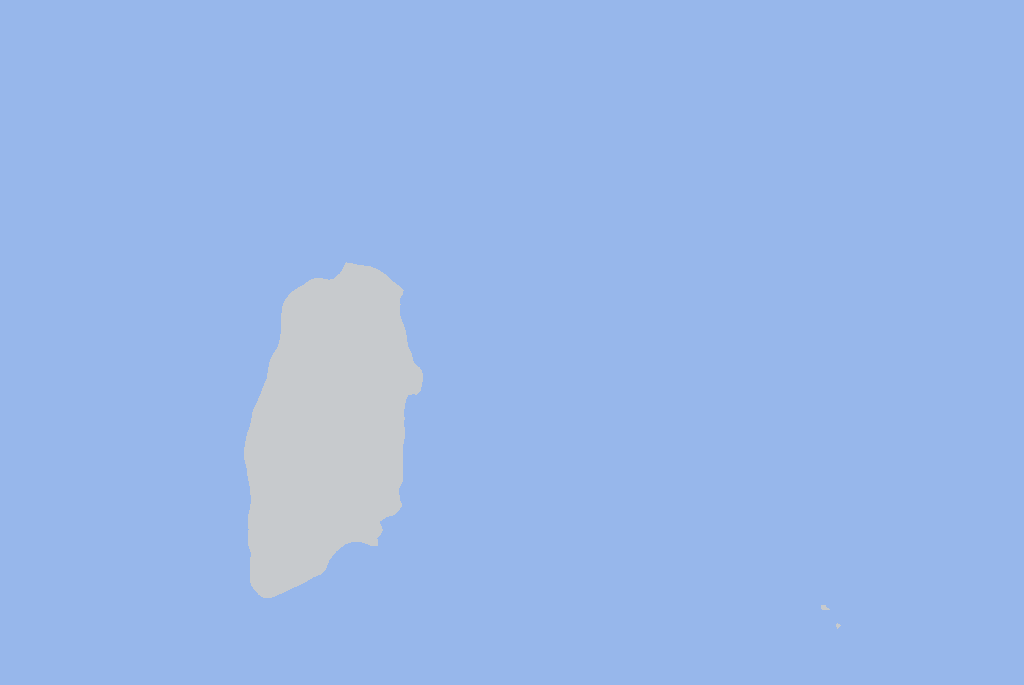
\includegraphics[width=\linewidth]{figures/COD10K_demo1/COD10K_demo1_pred_crf.png}
        \caption{DLabCRF}
    \end{subfigure}%
    \hfill
    \begin{subfigure}{0.25\textwidth}
        \centering
        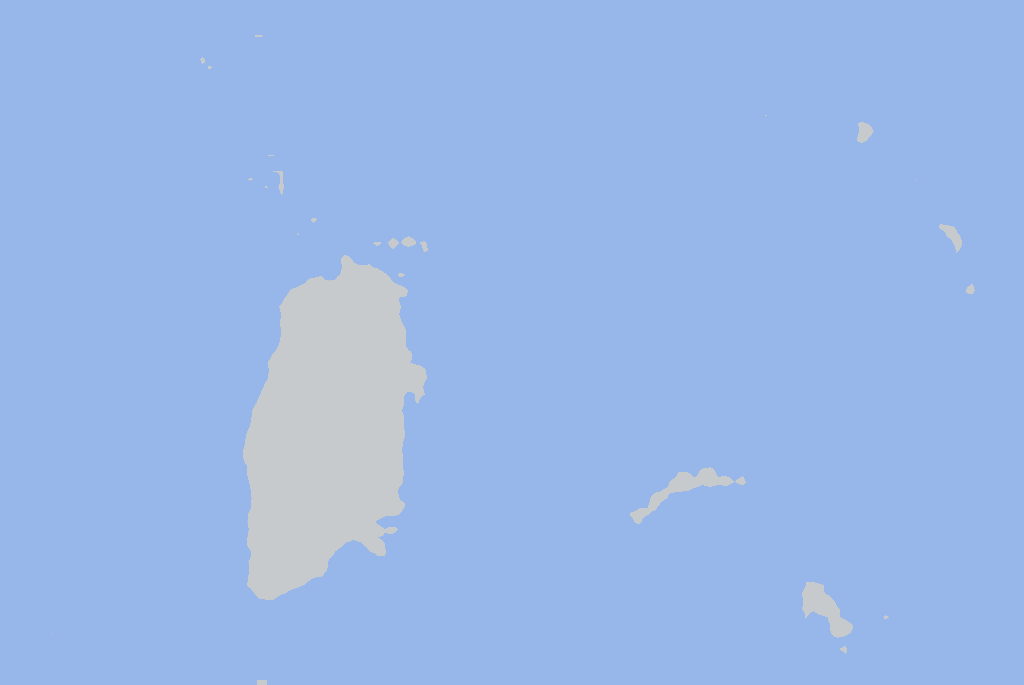
\includegraphics[width=\linewidth]{figures/COD10K_demo1/COD10K_demo1_pred_dlap.png}
        \caption{DLabSSVM}
    \end{subfigure}
    
    \caption{COD10K 可视化 \label{fig:COD10K_demo1}}
\end{figure}

我分别从CAMO Test和COD10K Test数据集中选取了一张图片进行可视化分析,从中可以看出分割效果最好的是DLabCRF模型,分割边界最平滑,分割区域集中,没有出现明显的误分类区域。
但其也没有完全能够恢复伪装目标的全部细节,比如图\ref{fig:COD10K_demo1}中的猫头鹰的耳朵部分就没有被分割出来。

DeepLab模型与DLabSSVM模型在可视化上可以看出有明显的误分割区域,但DeepLab模型的分割边界更加平滑,
DLabSSVM模型的分割边界更加锯齿化, 且DLabSSVM的误分割区域更多。


\subsection{伪装目标识别实验结果分析}



\section{附录}
\subsection{代码}


\bibliographystyle{plain}
\bibliography{references}

\end{document}